%\documentclass[10pt]{article}
\documentclass[conference]{IEEEtran}

%\usepackage{a4wide,setspace}
%\doublespacing
\usepackage{cite, graphicx, subfigure, amsmath, xspace, txfonts}
%\usepackage{eurosym} 

\newcommand{\us}{\,$\muup$s\xspace}

\begin{document}

\title{Processing Real-Time LOFAR Telescope Data \\ on a Blue Gene/P Supercomputer}
\author{John W. Romein and P. Chris Broekema and Jan David Mol and Rob V. van Nieuwpoort\\
Stichting ASTRON (Netherlands Institute for Radio Astronomy), Dwingeloo, The Netherlands\\
\small{\texttt{\{romein,broekema,mol,nieuwpoort\}@astron.nl}}}

\maketitle


\begin{abstract}
LOFAR is the first of a new generation of radio telescopes.
Rather than using expensive dishes, it forms a distributed sensor network that
combines the signals from many thousands of simple antennas.
Its revolutionary design allows observations in a frequency range that has
hardly been studied before.

This paper focusses on another novel feature of LOFAR: the approach to
process the real-time data in \emph{software}, where traditional telescopes
use customized hardware.
The use of software yields a much more flexible intstrument, but the high
processing and bandwidth requirements compel the use of a supercomputer.
The signals from the LOFAR stations are centrally combined, filtered, and
beamformed or correlated by a 10,880-core IBM Blue Gene/P system.

To meet the real-time requirements, the application is highly optimized.
Measurements show that we reach exceptionally high computational performance:
up to 96\% of the theoretical floating-point peak performance.
We also show that a major redesign of the network system software was
required to obtain enough internal I/O bandwidth to sustain the station data
streams and to greatly enhance flexibility that saves us on costs.
\end{abstract}


\section{Introduction}
LOFAR is an acronym for \emph{\textbf{LO}w \textbf{F}requency \textbf{AR}ray},
an aperture array radio telescope operating over the 10 to 250~MHz frequency
range.
It is the first of a new generation of radio telescopes, that breaks with
the concepts of traditional telescopes in several ways.
Rather than using large, expensive dishes, LOFAR uses many thousands of
simple antennas that have no moveable parts~\cite{Butcher:04,deVos:09}.
Essentially, it is a distibuted sensor network that monitors the sky
and combines all signals centrally.
This concept requires much more signal processing, but the additional costs
of silicon are easily offset by cost savings of steel.
Moreover, LOFAR can observe the sky in many directions concurrently and
switch directions instantaneously.
In several ways, LOFAR will be the largest telescope of the world, and will
enable groundbreaking research in astronomy and particle
physics~\cite{Bruyn:02}.

Another novelty is the elaborate use of \emph{software\/} to process
the telescope data in real time.
Previous generations of telescopes depended on custom-made hardware
because of the high data rates and processing requirements.
However, the desire for a flexible and reconfigurable instrument with
different processing pipelines for different observation types demands a
software solution.
The availability of sufficiently powerful supercomputers allows this.

This paper describes the implementation and performance characteristics of
the real-time part of some of these pipelines.
The standard imaging pipeline, used to generate sky images,
filters and correlates the data sent by the stations.
We present a highly-optimized implementation that achieves very high
computational performance: the correlator sustains 96\% of the theoretical
floating-point peak performance during the computational phase.
The Epoch-of-Reionization pipeline that should detect the faint, very first
sky objects, is a similar pipeline, but with even higher computational
demands, due to the increased amount of concurrent observation directions.
We describe several pulsar pipelines as well, that either search large sky
regions to find unknown pulsars or, once found, sensitively observe their
characteristics.
The pipelines share common components.
The software supports multiple concurrent observations. %, even of different types.

The telescopes produce hundreds of gigabits of data per second.
To handle the high data rate,
we use the Blue Gene in an unconventional way: we run \emph{application\/}
software on the so-called I/O~nodes to preprocess and postprocess data that are
further processed on the compute nodes.
This yields a very efficient system and, as we will show later, substantially
saved us on costs.
Since we were not able to achieve the required internal input and output data
rates with the standard network system software, we developed an extremely
low-overhead network protocol~\cite{Romein:09a}.

The remainder of this paper is structured as follows.
\emph{TODO}.


\section{LOFAR real-time central signal processing}
\label{sec:signal-processing}

CEP receives data from the stations via a dedicated wide-area network.
Each station locally combines the signals from its antennas and sends samples
to CEP.
A sample is a complex number that represents the amplitude and
phase of a signal at a particular time.
LOFAR supports $2\times4$, $2\times8$, and $2\times16$-bit samples.


\section{The Blue Gene/P}

Initially, LOFAR used a 6-rack IBM Blue Gene/L supercomputer for real-time
processing of the station data.
We recently replaced the system by an equally powerful 2.5-rack Blue Gene/P.
%The consequences of this upgrade are described in Section~\ref{sec:upgrade}.
Below, we describe the key features of the Blue Gene/P.

Our system contains 10,880 processor cores that provide 37.0~TFLOPS peak
processing power.
The system is built using SoC (System-on-a-Chip) technology that integrates
all processing and networking functionality on a single die.
One chip contains four PowerPC~450 cores, running at a modest 850~MHz clock
speed to reduce power consumption and increase package density.
Each core has two Floating-Point Units that provide support for
operations on complex numbers.
A core can sustain two fused multiply-adds per cycle.
The four cores share 2~GiB of main memory.
We use a configuration where we split the processor and memory into four
independent \emph{virtual nodes}.  %TODO: not here
This simplifies programming, since this allows single-threaded processing
on the compute nodes.  % TODO: tree is shared resource; mention?

The Blue Gene/P contains several networks.
A fast \emph{3-dimensional torus\/} connects all compute nodes and is used
for point-to-point and all-to-all communications.
The \emph{collective network\/} is used for MPI collective operations,
but also for external communication.
A \emph{global interrupt network\/} provides support for fast barriers.
Additional networks exist for initialization, diagnostics, and debugging.

Each compute node is connected to an I/O~node via the collective network
(see Figure~\ref{fig:pset}).
An I/O~node uses the same hardware as a compute node, but has its Ethernet
interface connected and runs another operating system (Linux).
Since our application demands high bandwidths, our system is configured with
the maximum number of 1~I/O~node per 16~compute nodes (64~cores).
The group of one I/O~node and the compute nodes that are connected to it,
is called a \emph{pset}.
Careful node allocation is necessary to schedule work on the right core
in the right pset.
The system has 160~psets in total.
Normally, the I/O~node is only used to provide transparent communication
from the compute nodes to external systems: all I/O-related system calls
on the compute nodes are forwarded to a daemon program that runs on the
I/O~node and performs the real operation.
In Section~\ref{sec:XXX}, we show how we can use the I/O~nodes much more
efficiently.


\section{LOFAR Processing}

\begin{figure*}
\includegraphics[width=\textwidth]{processing.pdf}
\caption{Simplified data flow diagram.}
\label{fig:processing}
\end{figure*}

The LOFAR station data are centrally processed in real time by a collection
of three distributed applications.
These applications run on different platforms:
the Blue Gene/P \emph{I/O nodes}, the Blue Gene/P \emph{compute nodes}, and on
external (PC-like) \emph{storage nodes}.
Figure~\ref{fig:processing} shows how the data flows through the entire
processing chain.
One application runs on the Blue Gene/P I/O nodes.
Its main tasks are to receive the station UDP data and to buffer the data
for up to 2.5~seconds.
The second application runs on the Blue Gene/P compute nodes, where the
compute-intensive processing takes place.
The main tasks are to reorder the data across the compute nodes over the
internal torus network, to filter the data, and to correlate or beamform
the filtered data.
The resulting data are then sent back to the I/O-node application, that
(in different threads) collects the data from the compute nodes and
sends the data to the storage nodes.
This is where the third application runs.
The storage nodes are PC-like systems with large disks.
The storage application collects the data from the I/O~nodes and writes the
data in some astronomical data format (AIPS++ Measurement Sets) to disk.

After an observation, bad data (due to interference) are removed, and the
resulting data are calibrated~\cite{Nijboer:07} and imaged.
This is done on off-the-shelf cluster hardware, and is not part of the
real-time processing system described in this paper.




%Sampled data can be invalid, for various reasons (e.g., because of
%radio interference, but also because of lost network packets).
Throughout the entire processing chain, we maintain which data is marked as
invalid (e.g, due to radio interference or due to lost UDP packets), so that
eventual images are not blurred by bad data.
Since invalid data is typically clustered, we use a \emph{SparseSet\/}
data structure that keeps a list of bad intervals.





\section{I/O-node processing}

%TODO real-time scheduling
%TODO best-effort buffers
We use the Blue Gene in an innovative way, by running application software
on the I/O~nodes.
On the Blue Gene/L, this required rewriting major parts of the system
software~\cite{Iskra:08}, but this idea is much better supported on the
Blue Gene/P.

We run one, multi-threaded process on each I/O~node that care of two tasks:
receipt and handling of the incoming station data, and handling of outgoing
output data.
Both tasks are described below.


\subsection{Input handling}

The FPGAs at a LOFAR station send UDP packets with sampled data over a
dedicated Wide-Area Network to a BG/P I/O~node.
To simplify the implementation, there is a one-to-one mapping between
stations and I/O~nodes, so that one I/O~node receives all data from a single
station.
However, handling the full 3.1~Gb/s data rate of a station on a relatively
slow CPU is quite a challenge.

The application receives the UDP packets, taking care of out-of-order,
duplicated, and lost packets.
Each station uses four FPGAs to send data to its associated I/O~node,
each FPGA to a different UDP port.
The I/O~node runs four ``input'' threads to receive a total of 48,828~packets
per second; one thread per socket.
Multiple threads are necessary, since a single core is insufficiently fast
to receive the data.

The received samples are copied into a cicular buffer that holds the most recent
2.5~seconds of data.
The buffer serves three purposes.
First, it is used to synchronize the stations, since the travel times over
the WAN are higher for the remote stations than for the central stations.
Second, the buffer prevents data loss due to small hiccups in the remainder
of the processing pipeline.
Third, the buffer is used to artificially delay the stream of samples,
as we will explain in Section~\ref{sec:delay-compensation}.
The buffer is limited by the small memory size, but due to good real-time
behavior of the application, 2.5~seconds is more than sufficient.

Another thread reads data from the circular buffer and sends the data to
the compute nodes for further processing.
It sends data in large bursts that contain approximately one second of samples.
We use \emph{FCNP (Fast Collective-Network Protocol)}, a newly developed
network library to efficiently communicate data between the I/O~nodes and the
compute nodes~\cite{Romein:09a}.
Existing network software did not provide sufficient bandwidths and consumed
too much CPU time.
FCNP, in contrast, achieves link-speed bandwidths for large messages, due to
its low overhead.
The data are sent directly from the circular buffer without additional copying.

Normally, when processing in real time, the NTP-synchronized wall-clock time
is used to trigger the sending of a new block of data.
A block of data containing samples from $t_1$ to $t_2$ are sent some hundreds
of milliseconds after $t_2$ (the WAN delay plus a safe margin), whether or
not all data were factually received from the station.
This ruthless method assures real-time continuation of the correlator and
provides fault-tolerance against a failing station or WAN link.
In practice, this method does not cause any data loss.
An alternative mode processes pre-recorded data off-line and is frequently used
for debugging and experimental observations.
In this case, the input is (reliably) read from file or TCP socket rather than
UDP.
Obviously, in off-line mode it is a bad idea to use the wall-clock time as
trigger, thus we synchronize the threads that read and write the circular
buffer differently to prevent them from overruning each other.


\subsection{Output handling}

The bulk of the signal processing is done on the compute nodes, on which we
elaborate in the next section.
The resulting output data are sent back to the I/O~node.
The second major task of the I/O-node application is to handle the output data.
This task performs four operations.

First, the data are received from the compute nodes, also using FCNP.
Second, the data are optionally added to previously received data from other
compute nodes in the pset, if integration over multiple seconds is desired.
Third, the (possibly integrated) output is queued in a buffer.
Fourth, another thread asynchronously dequeues the data and sends them to
a storage node, using a (reliable) TCP connection.

The queue improves real-time behavior and increases fault tolerance, since
it handles data on a best-effort basis.
If, for any reason, the data are not sent quickly enough to the storage node
(e.g., due to a disk or network failure), the queue fills up and subsequent
data are simply discarded until space is available.
This mechanism is important to keep the correlator running in real
time: it is much better to lose a small part of the data than to stall the
entire correlator and lose \emph{all\/} data.
In practice, under normal circumstances no data are lost.


\subsection{Performance}

Processing power on the I/O~nodes is a scarce resource, since most observation
modes are I/O bound.
Quite some optimizations were made to improve processing speed.
For example, the function that copies data from a received UDP packet to the
circular buffer is implemented in assembly, so that efficient 16-byte load and
store instructions (unknown to the C++ compiler) are used.
Unfortunately, the copy itself cannot be avoided, since a UDP packet contains
data of many frequency subbands that must be stored to different memory
locations.

Nevertheless, we first found that copying was very slow.
This was caused by the fact that the PowerPC~450 cannot handle
TLB\footnote{Translation Look-aside Buffer: a cache that caches
virtual-to-physical address mappings --- indispensable for efficient virtual
memory.} misses in hardware, but generates an interrupt and handles the fault
in software.
This is not a problem on the compute nodes, where the compute-node kernels 
map all memory using a few large pages, so that TLB misses do not occur.
However, the I/O~nodes run a Linux kernel that typically uses a page size of
4~KB, potentially generating huge amounts of TLB-miss interrupts.

To avoid the interrupts, we use a modified ZeptoOS (Linux-based)
kernel\cite{Kazutomo:09}.
It allows a process to map 1.5~GiB (out of 2~GiB) of physical memory in its
virtual memory map, using six fixed mappings of 256~MiB that are never evicted
from the TLB.
Hence, this memory does not generate TLB misses.
The remainder of the memory is used for normal, paged operation.
The application uses this fast memory for the circular buffer and for the
output queues.
Copying data from received UDP packets to the input buffer is up to five times
faster than using paged memory.

To achieve good real-time behavior, we found that it is of utmost importance
to carefully manage thread priorities using the Linux real-time scheduler.
Since the compute nodes must always be able to proceed, they must be fed with
data without delays.
Therefore, the thread that sends data from the circular buffer to the
compute nodes runs at the highest priority, and is scheduled as soon as the
wall-clock time triggers.
The thread that reads results from the compute nodes is almost equally
important, since compute nodes will not accept new work before the previous
results were read by the I/O~node.
Other threads, such as the threads that read UDP data and the threads that
send data from the output queues are also important, but if they would ever
fail to meet a real-time deadline, only a small amount of data is lost.
In practice, under normal circumstances, this happens close to never.





\section{Compute-node processing}

\begin{figure}
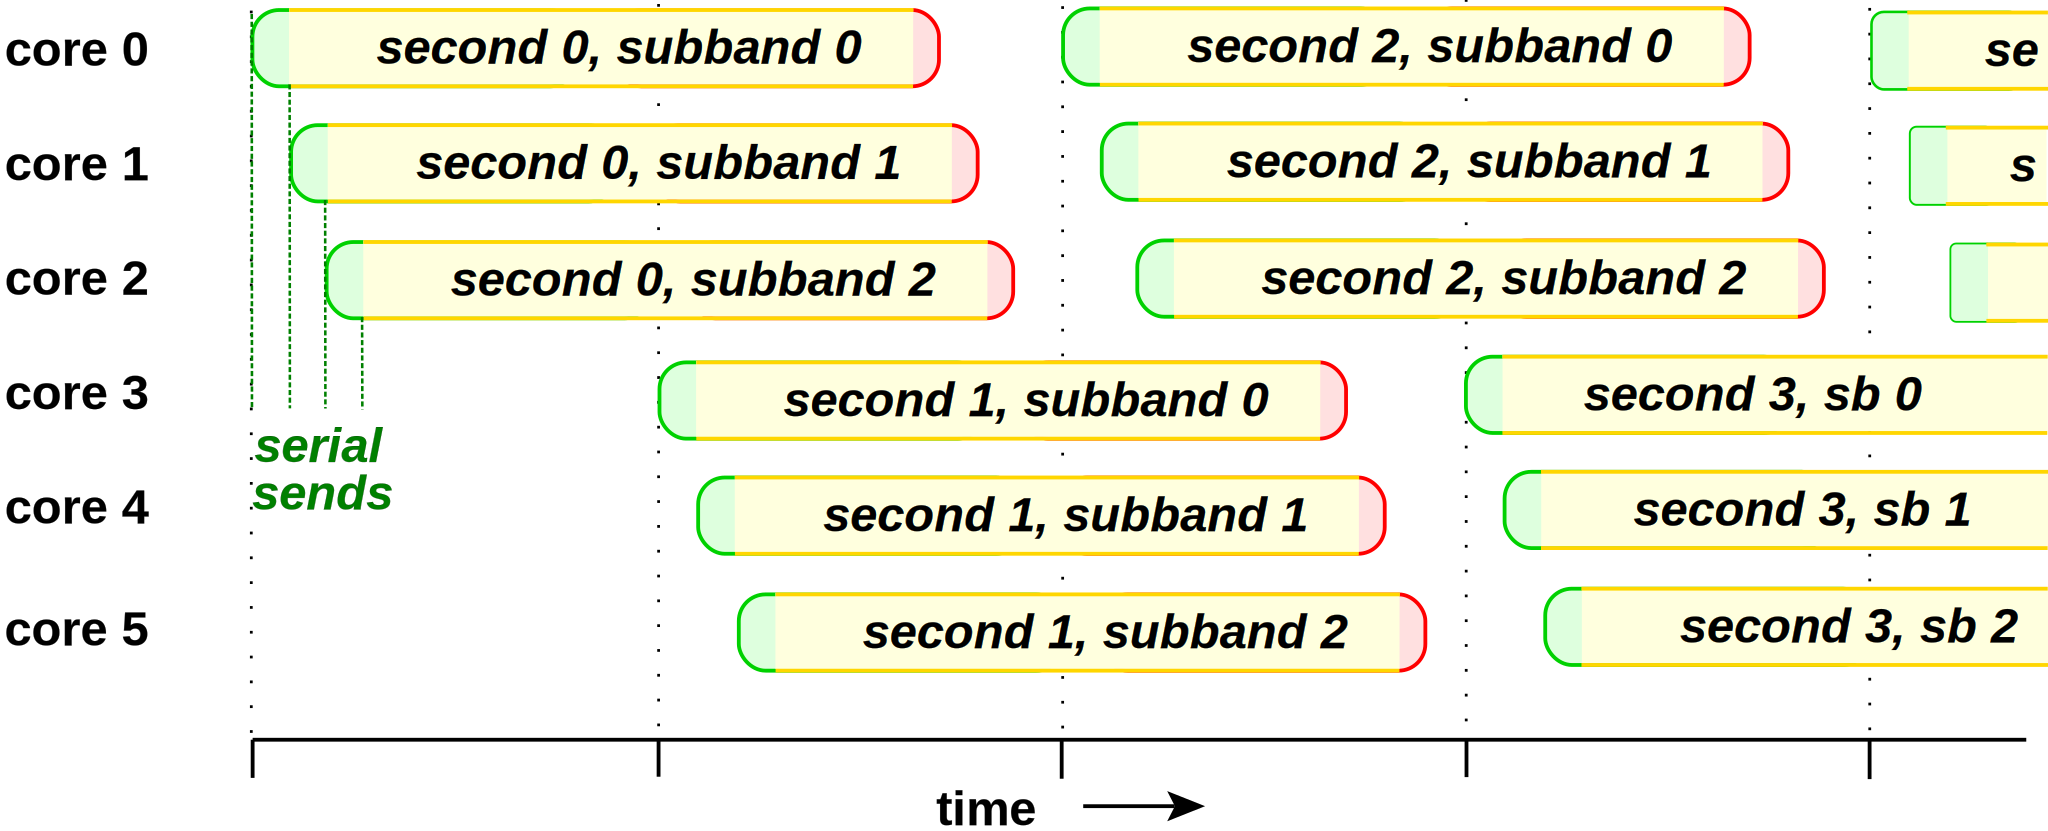
\includegraphics[width=\columnwidth]{round-robin.pdf}
\caption{Round robin processing of work over compute-node cores.}
\label{fig:round-robin}
\end{figure}

The I/O~node chops the stream with station data into chunks of one frequency
subband and approximately one second time.
Since processing such a chunk typically takes much more than one second,
the chunks are round-robin distributed over a group of processor cores,
as illustrated by Figure~\ref{fig:round-robin}.
Subsequent chunks of data are processed by different processor cores.
A core must finish its work before it is time to process the next chunk of data.
A core first receives data from the I/O~node (green in the figure),
processes them (yellow), sends back the results (red), and idles until the
I/O~node sends new data.

In reality, the scheduling is more complicated than shown in
Figure~\ref{fig:round-robin}, because the 64~cores in a pset are typically
resposible for processing four to sixteen subbands, rather than one.
For example, if a pset needs to process six subbands, every second, the next
six cores are scheduled and each of them will process one subband.

The compute node performs quite some operations on the data, as shown in
Figure~\ref{fig:processing}.
The very first step is to exchange data with other groups of processor cores.
This is necessary, because an I/O~node receives all frequency subbands from one
station, but the correlator (see below) requires one frequency subband from all
stations.
The data exchange is challenging, since it involves hundreds of gigabits per
second.
We use the 3-D~torus because of its high bandwidth and switching capabilities.

Unfortunately, an I/O node cannot send the data directly from the circular
buffer to the compute core that will process the data, since the I/O~node is
only connected to the compute nodes in its own pset.
The data are thus first sent over the collective network from the I/O~node to
a compute node and then over the 3-D~torus.

The torus bandwidth between colinear and coplanar nodes is lower than between
non-coplanar nodes, since non-coplanar nodes communicate over more links
(in three dimensions) simultaneously.
Therefore, we schedule work that needs exchange of data as much as possible
on non-coplanar cores.
We also avoid situations where multiple cores of the same processor need to
access the torus or collective network simultaneously, since these resources
are shared and simultaneous access decreases performance.
The code that implements the data exchange and scheduling are, in the presence
of many stations, many subbands, time slicing, round-robin core allocation,
and avoidance of resource conflicts, \emph{extremely\/} complicated, but
highly efficient.

On the BG/L, the data exchange was implemented synchronously, using
\texttt{MPI\_Alltoallv()}.
The BG/P, in contrast, uses DMA for the torus, allowing asynchronous
communication.
We re-implemented the data exchange using asynchronous point-to-point
communication, that overlaps communication with the next four processing steps.
As soon as a chunk of data from one station has arrived, the core starts
processing them, up to the point that the data from \emph{all\/} stations
are required.

\subsection{Signal Processing}

After the data exchange, a core possesses the samples of one subband, from all
stations.
The data are processed through a number of filters, as briefly described below.
More details on most filters (except bandpass correction and beam forming)
can be found elsewhere~\cite{Romein:06}.

The subband data are first filtered by a \emph{Poly-Phase Filter\/} (PPF) that
splits a frequency subband into narrow frequency channels, trading time
resolution for frequency resolution.
The high frequency resolution allows for removal of narrow-band
\emph{Radio Frequency Interference\/} (RFI, e.g., caused by TV transmitters)
later in the pipeline.
Typically, a 195~KHz subband is split into 256~channels of 763~Hz, but the
filter supports any (reasonable) power-of-two number of channels.

As a side effect, the PPF implicitly converts 16-bit, little-endian, integer
samples to 32-bit, big-endian floating point numbers, since the Blue Gene is
much better at floating-point processing than integer processing.
Since this doubles the data size, the PPF runs \emph{after\/} the data
exchange.
The PPF itself consists of a number of 16-tap Finite Impulse Response (FIR)
filters, of which the output are Fourier Transformed.
The FIR filters and a 256-point FFT are implemented in assembly, for optimal
performance.
For other FFT sizes, we use the Blue Gene ``Vienna'' version of
FFTW~\cite{Lorenz:05}.

The next step is to artificially ``delay'' the stream of station samples,
to compensate for the fact that a celestial wave hits stations at different
times~\cite[Sec.~2.1]{Romein:06}.

The next step is to artificially ``delay'' the stream of station samples.
Due to the finite speed of light, the wave from a celestial source hits
stations at different times, depending on the observation direction, the
station positions, and the rotation of the earth~\cite[Sec.~2.1]{Romein:06}.
Before the signals can be correlated, all station streams are aligned.
XXX
For example, a delay of 22\us can be achieved by shifting four 5.12\us
samples and a frequency-dependent phase rotation that compensates the
remaining 1.52\us.
The phase rotation itself costs a complex multiplication per sample.
The delays are computed exactly once per second and interpolated in frequency
and time for each individual sample.

The next step is a bandpass correction that compensates for an artefact
introduced by a station filter (the PPF that creates subbands).
Without correction, some channels contain more power than others.
The correction is performed by multiplying each complex sample by a real,
channel-dependent value that is computed in advance.
A station cannot correct for this artefact itself, since it is only visible
in channels, not in subbands.

Although the FIR filters, FFTs, delay compensation, and bandpass correction
are conceptually separate, consecutive blocks, their implementations are
highly interweaved to achieve better performance.
This avoids that four separate passes over all data are made.
Also, many of the computations are hidden by the memory access delays that
are the result of a transpose in main memory.



\subsection{Performance}

For optimal performance, most time-intensive code is written in assembly,
because the performance from compiled C++ code was by far not sufficient.
We maintain equivalent C++ reference code for testing and portability.
The assembly version hides load and instruction latencies, issues concurrent
floating point, integer, and load/store instructions,
and uses the L2 prefetch buffers in the most optimal way.
Most instructions are parallel fused multiply-adds, that sustain four
operations per cycle.



%Although the correlator (including the other signal-processing steps) is a
%typical example of a streaming-data application, the perception ``byte goes
%in, byte comes out'' is misleading.
%The data are necessarily cut into large chunks, and basically every processing
%step needs the data in another order than the previous step produced.
%This maps poorly to the memory subsystem, that is not optimized for
%non-consecutive memory accesses.
%We also found that the round-robin replacement algorithm of the L1 caches
%XXX





%\section{I/O performance}

%The stations produce large amounts of data.
%The LOFAR specification requires 32~MHz of observation bandwidth with 16-bit,
%dual-polarized complex samples, yielding 2.1~Gb/s per station.
%However, both the station hardware and the Wide-Area network are capable of
%handling more data, up to 3.1~Gb/s per station.
%Also, some stations can be geographically split into two halves, doubling the
%data rate, but we treat both halves as separate stations, so that the number
%of stations increases but the data rate per station remains the same.

%As supercomputers are usually not optimized for external I/O, streaming data
%into the correlator at these rates is challenging.
%One of the reasons to choose for the Blue Gene as correlator was its atypical
%high number of external GbE interfaces, 768 in six racks.

%Despite its potential, streaming data into the machine at the required rates
%turned out to be problematic~\cite{Romein:06}.
%Each GbE interface has to sustain at least 550~Mb/s in and 200~Mb/s out
%(concurrently) to keep up with the stations.
%Initially, the total bandwidth (in and out) obtained in practice peaked at
%about 300~Mb/s.
%After a year of updating drivers and tuning parameters, aggregate bandwidths
%of about 850~Mb/s were seen, provided that four (out of sixteen) compute nodes
%communicated concurrently through the same I/O~node, effectively wasting
%3/16$^\mathrm{rm}$ of all compute resources.
%Also, the higher data rates were only seen using benchmark programs; the
%application exhibits more complex communication patterns that had a
%devastating impact on the performance.


%Although the BG/P is computationally very efficient,
%streaming the station data into the machine at the required data rates
%turned out to be a major problem in practice~\cite{Romein:06},
%despite the high number of I/O interfaces.
%For each 64~BG/P compute cores, there is one \emph{I/O~node\/} that
%has one external gigabit-Ethernet interface and transparently handles all I/O
%calls initiated by its associated compute cores through system call function
%forwarding (see Figure~\ref{fig:IOnode}).
%We found that the stock network system software was not particularly optimized
%for high-throughput I/O, and that the obtained bandwidths were insufficient
%for LOFAR operation.

%The dissatisfaction about the performance and about the I/O model in general
%led to a joint effort to redesign the entire network software infrastructure,
%and resulted in a new environment called {\em ZOID\/}~\cite{Iskra:08}.
%ZOID does not only yield better performance, but it is much more flexible,
%since it allows application code to be run on the I/O~node.
%With ZOID, we were able to move the receipt of the station data from the input
%cluster nodes to the BG/P I/O~nodes, so that the station data are sent
%directly through the WAN into the BG/P.
%Not having to build a separate input cluster results in an estimated cost
%saving of \euro700,000.




%\section{Upgrading from a BG/L to a BG/P}
%\label{sec:upgrade}
%
%Recently, the six-rack Blue Gene/L system was replaced by a 2.5-rack Blue
%Gene/P system, that provides approxiamately the same computational power.
%The biggest improvements of the BG/P over the BG/L are summarized below.
%First, the number of cores in a processor and the speeds of the processors and
%networks have increased.
%Second, the L1 caches are, unlike those of the BG/L, coherent.
%Third, the 3-D torus is extended with a DMA controller that allows
%asynchronous communication.
%Fourth, its programming environment has greatly improved; many System
%Programming Interfaces and part of the system software has become open source.
%Fifth, the 1-GbE technology of the BG/L was replaced by 10-GbE technology.
%Furthermore, there are improvements in reliability and power consumption.
%
%The improved programming environment and the change to 10-GbE technology
%had significant implications for our application.
%While the amount of FLOPS per rack has become 2.43 as high, the number of
%external interfaces has halved.
%As a consequence, each I/O~node has to handle (at least) four times as much
%data as on the BG/L.
%However, the total processing power on the BG/P has only improved by a factor
%of 2.43, while the load on the I/O~nodes of the BG/L was already problematic!
%Also, we measured that the link speed of the collective network that connects
%the I/O~node to the compute nodes cannot carry more than 6.54~Gb/s payload.
%%Taking the high costs of the UDP/IP protocol stack into account, we thought
%%that handling the full station data rate of 3.1~Gb % FIXME
%
%

\section{Results}

\begin{figure}
\includegraphics[width=\columnwidth]{fringe.jpg}
\caption{``Fringes'' from a 9-hour observation.  The phase of the correlated
signal (represented by color) changes due to the earth rotation that alters
the relative position of the observed source.
The white spots are caused by interference; these data are ignored in the
remainer of the processing pipeline.}
\label{fig:fringe}
\end{figure}


\section{Performance}

Since only a small number of LOFAR stations has already been constructed
(the majority will become operational later this year), we will provide 
realistic performance measurements with externally generated dummy data.
We use one rack to generate UDP data, another rack for the correlator, and
the remaining half rack to receive (and dump) the correlated data.
The simulation is very realistic, since the correlator runs exactly
the way it would run with real station data.

With one rack, we can process up to 64~stations, one per I/O~node.



\subsection{Computational performance on the I/O Nodes}

\begin{figure}
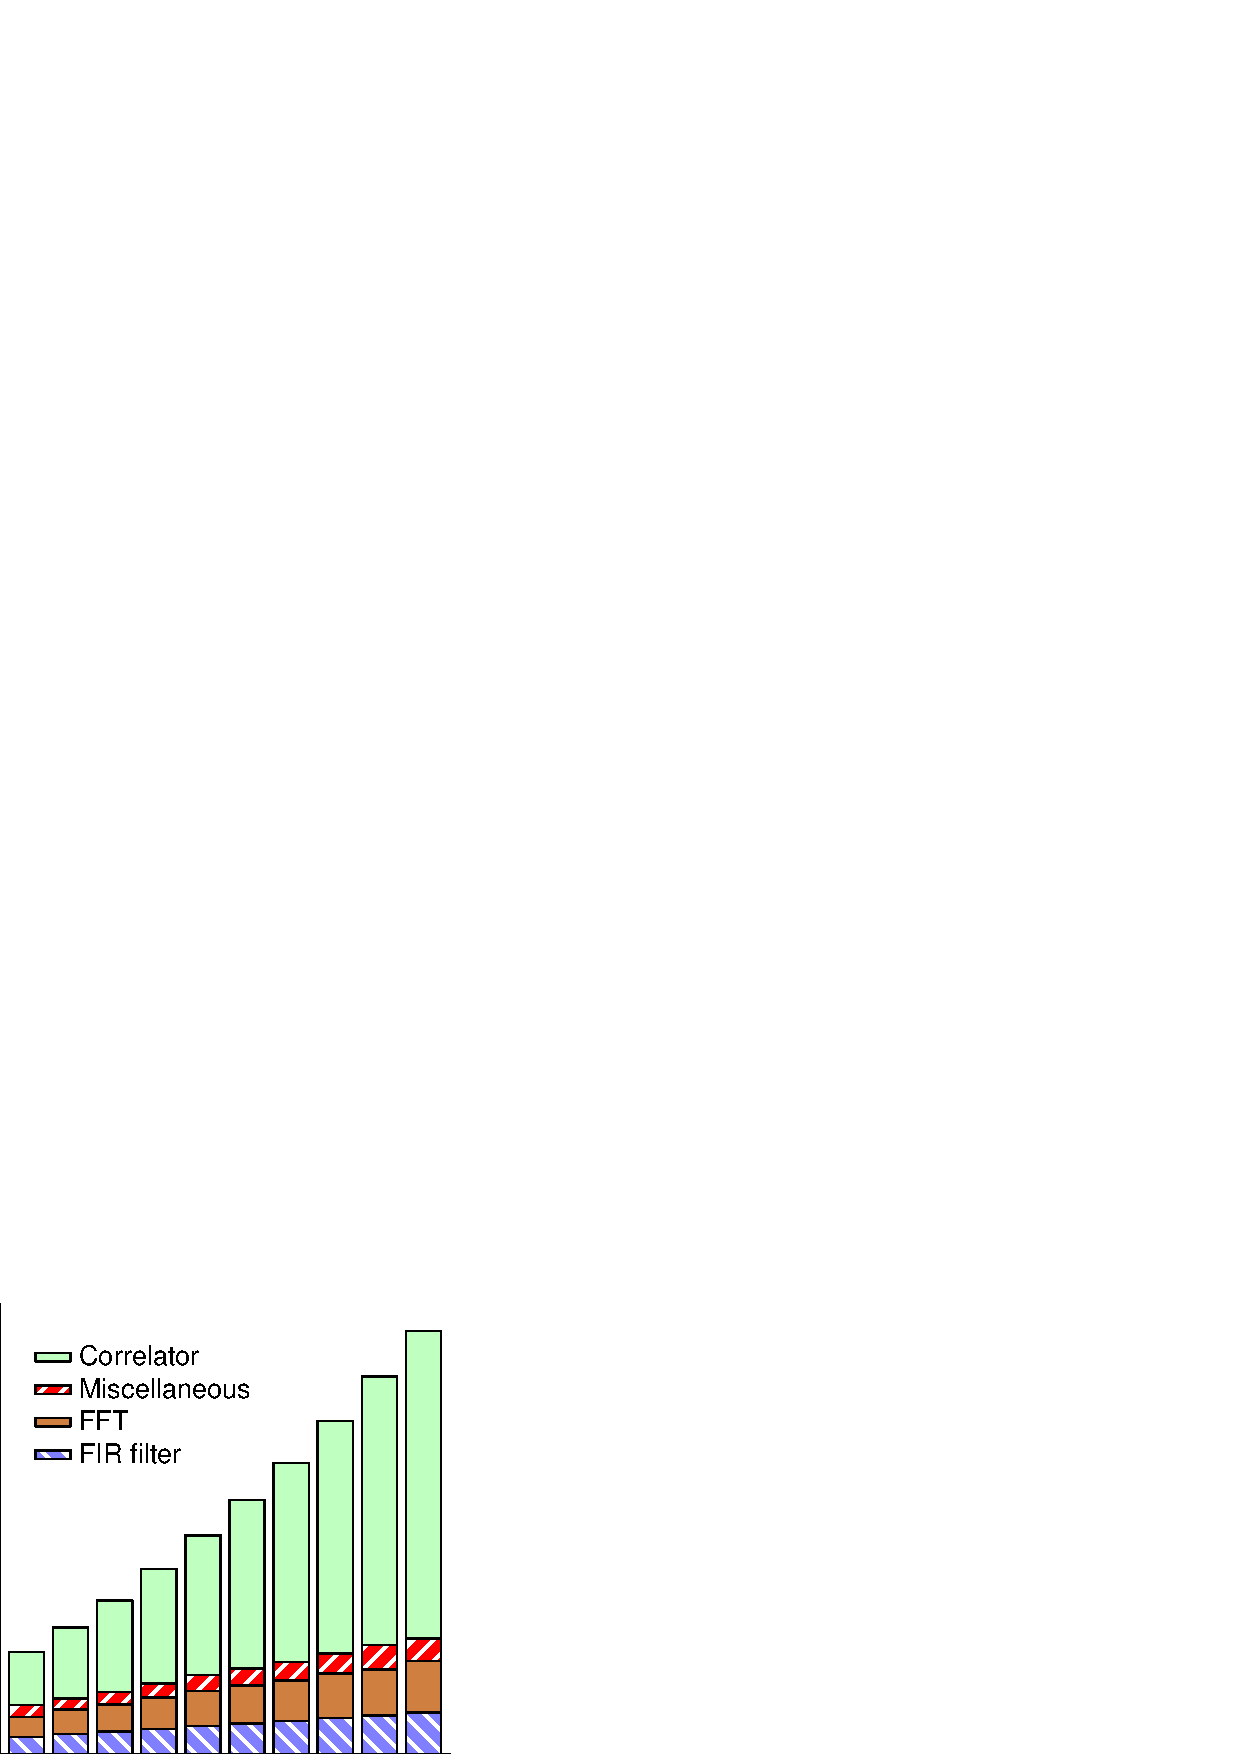
\includegraphics[width=\columnwidth]{speed.pdf}
\caption{I/O Node performance breakdown (248~subbands).}
\label{fig:ionode-load}
\end{figure}

The I/O node application is optimized so thoroughly that it can receive a
station input of 3.1~Gb/s --- 51\% above the LOFAR requirements; the
absolute maximum that a station can generate.
Additionally, an I/O node sends up to 580~Mb/s to storage.
Figure~\ref{fig:ionode-load} shows where an I/O~node spends its time.
Even at these data rates, the idle time is 34\%, more than sufficient for
smooth, real-time handling of data.

The most time-consuming operation (36\%) is the receipt of UDP packets by
the kernel, as each I/O~node receives 48,828~UDP packets of 7,998~bytes
per second.
Copying the received data to the circular buffer adds 7\% to the load.
FCNP efficiently forwards the data directly from the circular buffer to the
compute nodes~(15\%) and receives the correlated data from the compute
nodes~(3\%).
Sending the data to the storage nodes (over TCP) takes~5\%.
Other tasks have negligible impact on the processor load.

Both FCNP and the fixed TLB mappings significantly contribute to the low
resource usage.
Without either of them, the application cannot handle these data rates in
real time.
If future observation modes would require higher output data rates, we may
optimize the memory copy routines in the Linux kernel by using the
Blue-Gene-specific 16-byte load/store instructions, rather
than standard 4-byte PowerPC load/stores.
We think this will reduce the system time of I/O operations.


\subsection{Computational performance on the Compute Nodes}

The load on the compute nodes depends heavily on the observation parameters.

Most of the observations can be done using only one rack of Blue Gene/P.
This small amount of resources 


\section{Conclusions and future work}



% Future work: RFI, online calibration, other pipelines


\section*{Acknowledgments}

We thank Ger van Diepen, Martin Gels, Marcel Loose and Ruud Overeem
for their contributions to the LOFAR software.
We also thank Kamil Iskra and Kazutomo Yoshii from Argonne National Laboratory
for their work on ZOID and ZeptoOS.
Todd Inglet, Tom Liebsch, and Andrew Taufener from IBM Rochester provided the
necessary support to optimally use the Blue Gene/P.

LOFAR is funded by the Dutch government in the BSIK programme for
interdisciplinary research for improvements of the knowledge infrastructure.
Additional funding is provided by the European Union, European Regional
Development Fund (EFRO) and by the ``Samenwerkingsverband Noord-Nederland,''
EZ/KOMPAS.

\bibliographystyle{plain}
\bibliography{lofar}

\end{document}
